\chapter{Firmware and Testing}

\graphicspath{{./Figures/Firmware and Testing/}}
In this chapter, the firmware development process is detailed, including the programming languages and tools used, the integration with hardware, and the testing framework and methodology.
The test cases and scenarios are presented, along with the results of the testing procedures.
Finally, the process of debugging and troubleshooting encountered problems is discussed.

%\begin{itemize}
%	\item Overview of the chapter's content and its significance in the context of the overall project.
%	\item Briefly state the objectives of firmware development and testing procedures.
%\end{itemize}
\newpage

\section{Firmware Development}
%\begin{itemize}
%	\item Discuss the development environment and tools used for firmware programming.
%	\item Detail the architecture and design of the firmware, including flowcharts or state  diagrams if applicable.
%	\item Explain the implementation of key functionalities such as control algorithms, sensor integration, and actuator management.
%\end{itemize}
\section{Programming Languages and Tools}
%\begin{itemize}
%	\item List and describe the programming languages used for firmware development.
%	\item Mention any specific software tools, libraries, or frameworks employed.
%\end{itemize}
Mainly, the firmware is written in C language, with some parts written in C++.The STm32CubeIDE is used as the IDE for the firmware development.
Using the Cube IDE, the STM32CubeMX is used to generate the initialization code for the microcontroller.
%figure for the Pinout & Configuration
\begin {figure}[h]
\centering
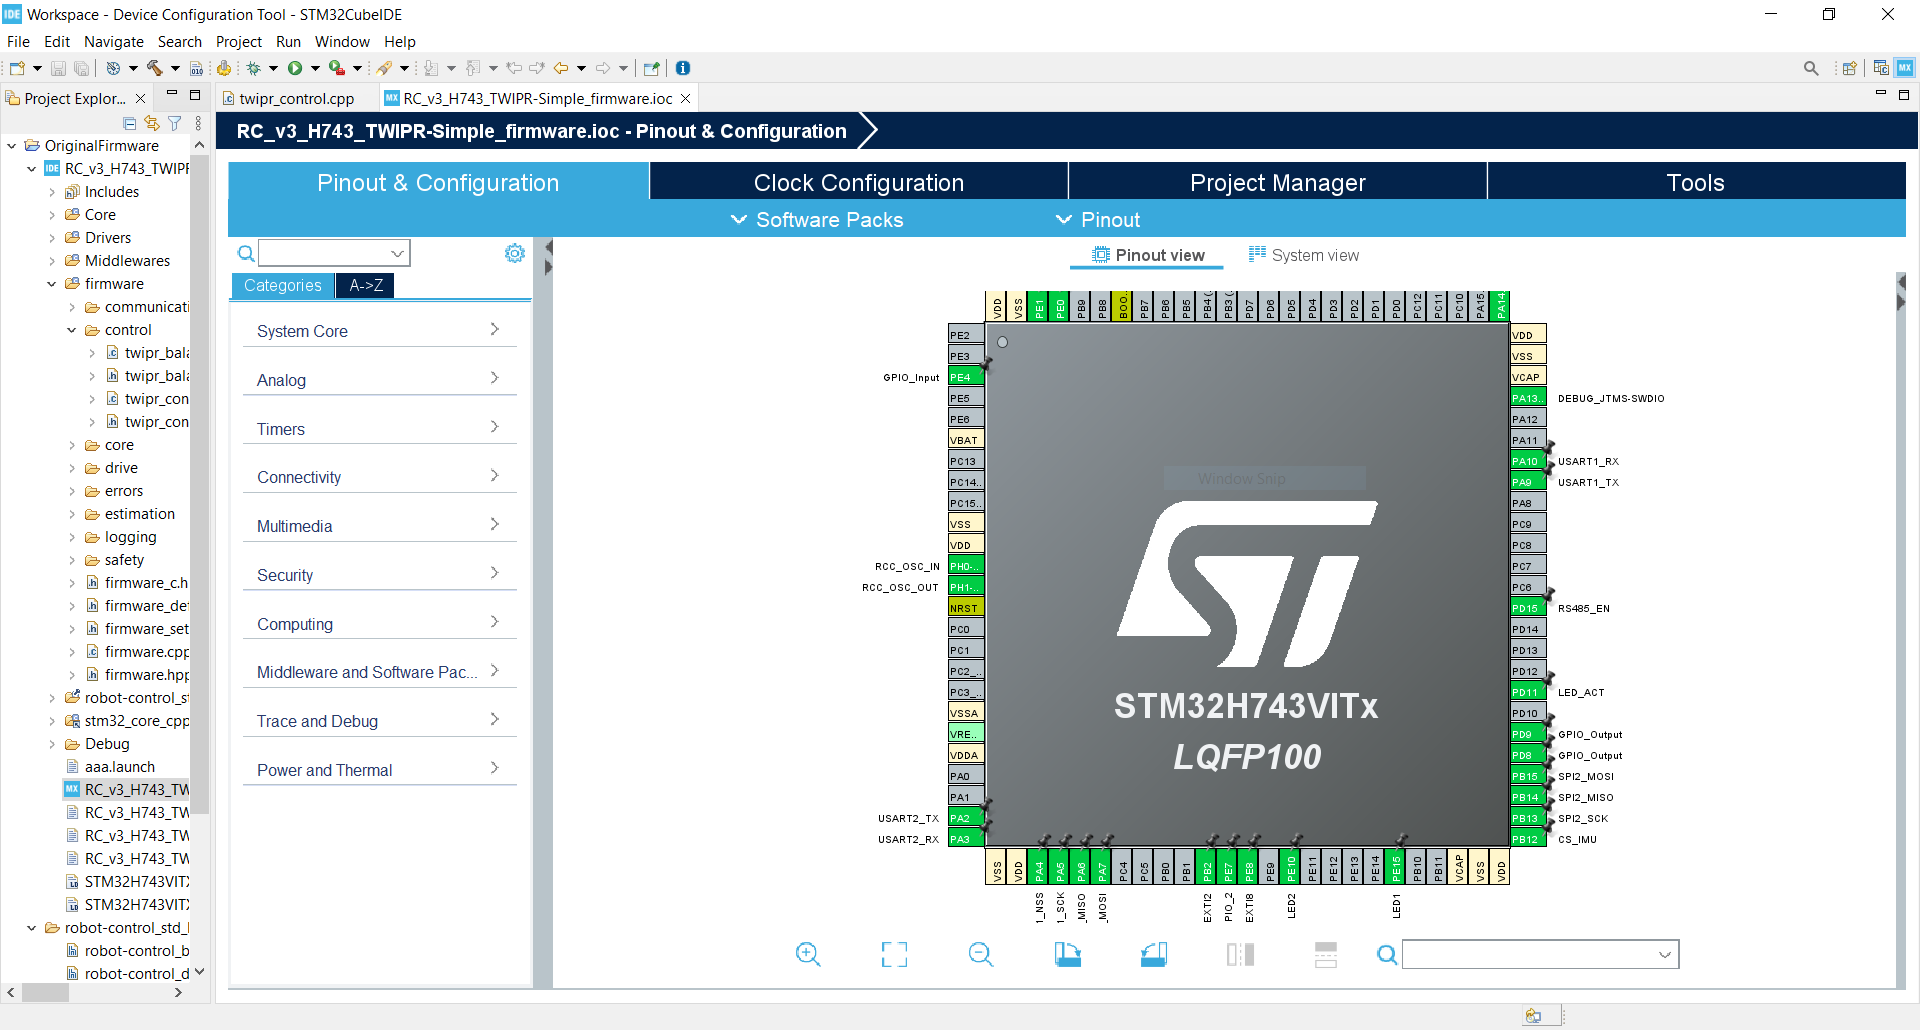
\includegraphics[width=.8\textwidth]{Pinout & Configuration}
\caption{Pinout \& Configuration}
\label{fig:Pinout}
\end {figure}

The stm32CubeIDE can configure the microcontroller peripherals, such as the GPIOs, timers, and UART. After configuring the microcontroller, the STM32CubeIDE generates the initialization code for the user.
%figure for the clock confugration
\begin {figure}[h]
\centering
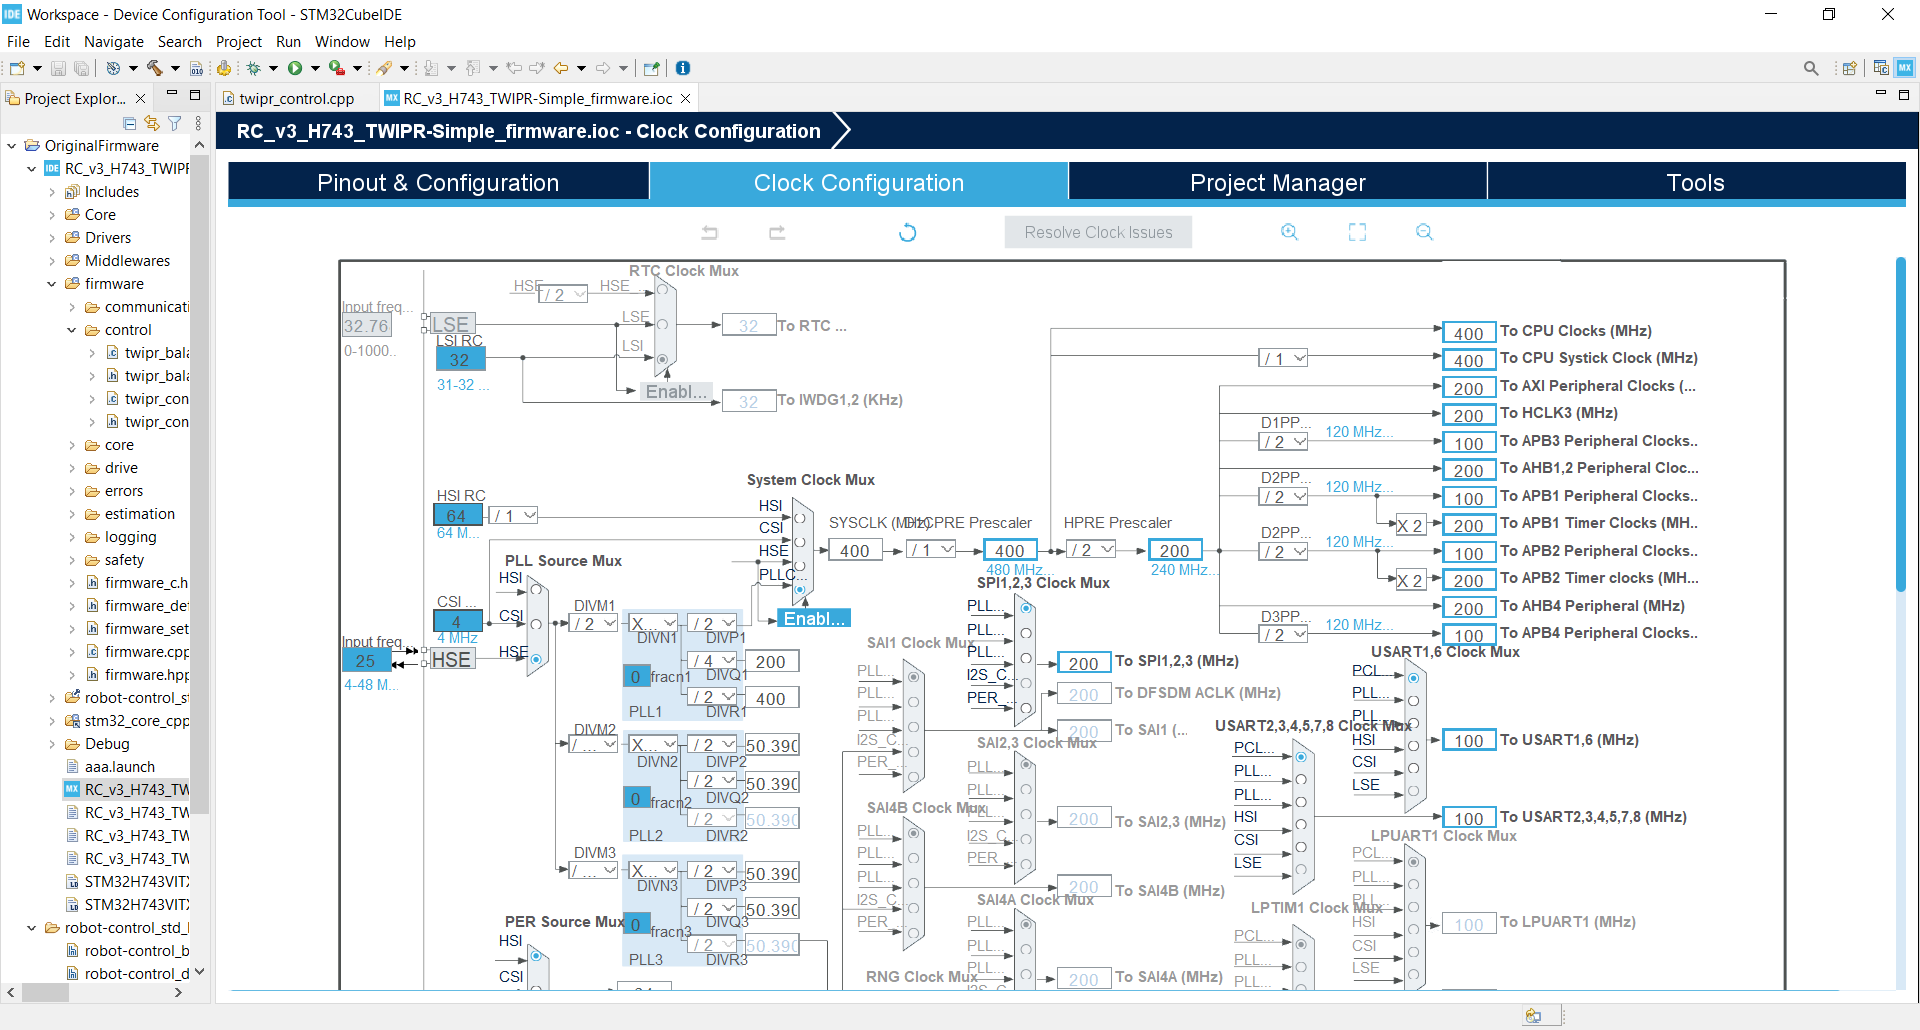
\includegraphics[width=.8\textwidth]{Clock Configuration}
\caption{Clock Configuration}
\label{fig:clock}
\end {figure}

The STM32CubeIDE allows clock configuration for the microcontroller.


The STM32Cube also generates the Makefile for the project, which is used to compile the firmware.
The STM32CubeIDE is used to compile the firmware and upload it to the microcontroller.
The STM32CubeIDE is based on the Eclipse IDE, which is an open-source IDE.


Python is also used to pass the control parameters to the microcontroller using the UART. The wireless SSH connection allows the user to change the control parameters without the need to connect the microcontroller to the computer as long as the raspberry pi and the pc are connected to the same network.

\section{Integration with Hardware}
The robot hub Board is used to connect the microcontroller to the sensors and actuators. It also provides the power supply for the microcontroller as well as acting as a carrier board for raspberry pi.
The robot hub board allows using the full potential of the microcontroller by providing the necessary connections.
%\begin{itemize}
%	\item Discuss how the firmware interacts with and controls the hardware components.
%	\item Explain any challenges encountered in integration and how they were resolved.
%\end{itemize}
\section{Testing Framework and Methodology}
%\begin{itemize}
%	\item Outline the testing framework used to validate the firmware.
%	\item Describe the methodology for functional testing, including unit tests, integration tests, and system-level tests.
%\end{itemize}
\section{Test Cases and Scenarios}
%\begin{itemize}
%	\item Present the results of the testing procedures.
%	\item Analyze these results, highlighting successful areas and identifying any issues or bugs discovered.
%\end{itemize}
\newpage
\section{Debugging and Troubleshooting}
%\begin{itemize}
%	\item Discuss the process of debugging and troubleshooting encountered problems.
%	\item Explain how issues were diagnosed and resolved.
%\end{itemize}
%figure for Jlink
\begin {figure}[h]
\centering
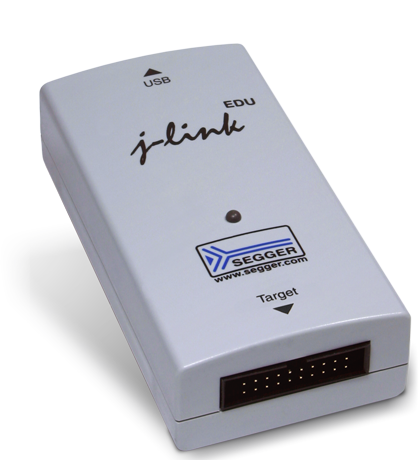
\includegraphics[width=0.5\textwidth]{jlink}
\caption{Jlink Debugger}
\label{fig:Jlink}
\end {figure}


Jlink is used to upload the firmware to the microcontroller.
As well as debugging the firmware.
The Jlink is a hardware debugger that connects to the microcontroller using the SWD interface.
The Jlink allows debugging breakpoints and stepping through the code.


